\documentclass[../report.tex]{subfiles}
\begin{document}

\graphicspath{{img/}{../img/}}

\subsection{Business Logic Layer Design}



\begin{landscape}

\newgeometry{left=1cm,right=-3cm}

\subsection{Class Diagram}

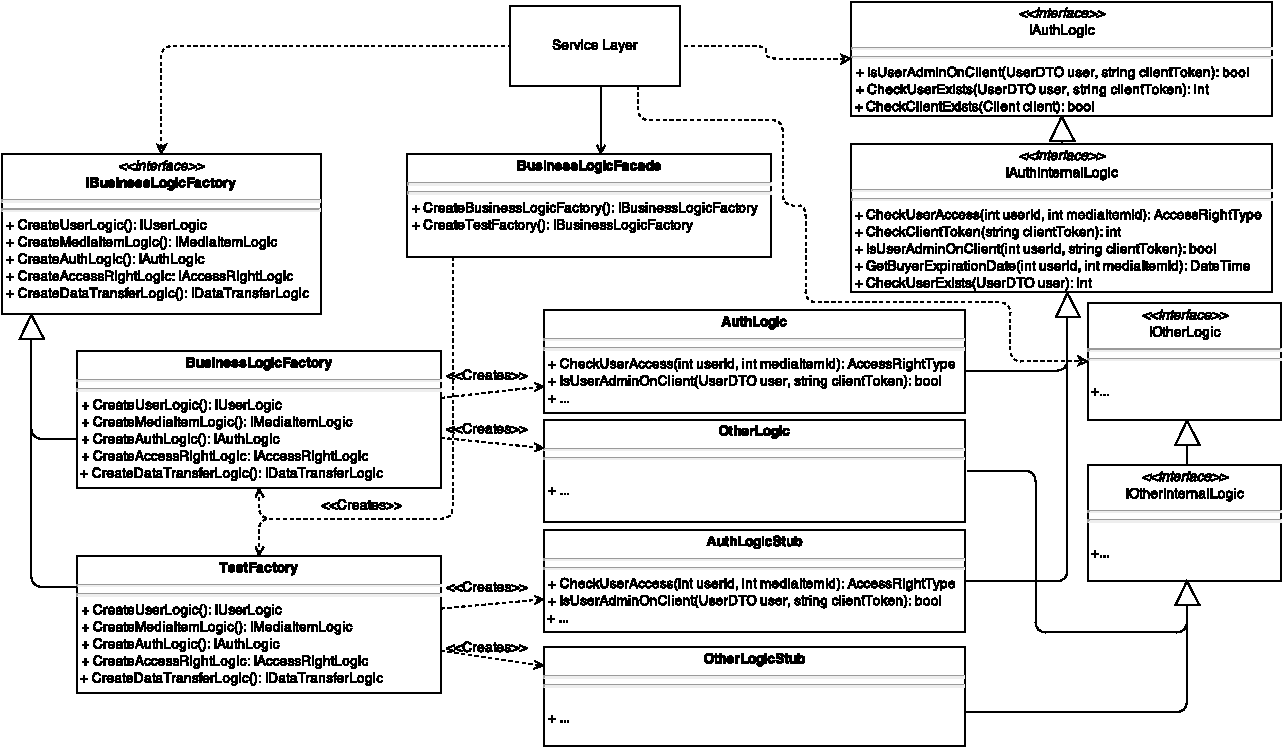
\includegraphics[ scale=1.2]{BusinessLogicLayerDiagram.pdf}

\end{landscape}

In our Business Logic Layer we use an Abstract Factory pattern with Facade pattern on top to provide easy interaction between the Service Layer and the Business Logic Layer. The idea of the Facade Pattern is to only expose a single concrete class which in our case is the BusinessLogicFacade class. The BusinessLogicFacade class makes it possible to get hold of the concrete factories without exposing the factories themselves to the Service Layer.

Underneath the Facade pattern lies the Abstract Factory pattern which starts with the Abstract Factory interface which in our case is the IBusinessLogicFactory. This interface specifies a method for creating each of the Abstract Products in this Abstract Factory. The Abstract Products are IAuthLogic, IUserLogic, IMediaItemLogic, IAccessRightLogic and IDataTransferLogic. We then have two concrete implementations of this interface and those are the BusinessLogicFactory and the TestFactory classes. Each of the concrete factories can then produce an instance of a concrete implementation of each Abstract Product. These concrete implementations must implement the Abstract Product interface which contains the methods that are exposed to the Service Layer. But they must also implement an internal interface (ie. IAuthInternalLogic) which specifies methods that are used internally in the Business Logic Layer. These internal interfaces make it possible for the different concrete logic classes to expose methods to one another but not to the Service Layer.

\end{document}